\documentclass[twoside]{book}

% Packages required by doxygen
\usepackage{fixltx2e}
\usepackage{calc}
\usepackage{doxygen}
\usepackage[export]{adjustbox} % also loads graphicx
\usepackage{graphicx}
\usepackage[utf8]{inputenc}
\usepackage{makeidx}
\usepackage{multicol}
\usepackage{multirow}
\PassOptionsToPackage{warn}{textcomp}
\usepackage{textcomp}
\usepackage[nointegrals]{wasysym}
\usepackage[table]{xcolor}

% Font selection
\usepackage[T1]{fontenc}
\usepackage[scaled=.90]{helvet}
\usepackage{courier}
\usepackage{amssymb}
\usepackage{sectsty}
\renewcommand{\familydefault}{\sfdefault}
\allsectionsfont{%
  \fontseries{bc}\selectfont%
  \color{darkgray}%
}
\renewcommand{\DoxyLabelFont}{%
  \fontseries{bc}\selectfont%
  \color{darkgray}%
}
\newcommand{\+}{\discretionary{\mbox{\scriptsize$\hookleftarrow$}}{}{}}

% Page & text layout
\usepackage{geometry}
\geometry{%
  a4paper,%
  top=2.5cm,%
  bottom=2.5cm,%
  left=2.5cm,%
  right=2.5cm%
}
\tolerance=750
\hfuzz=15pt
\hbadness=750
\setlength{\emergencystretch}{15pt}
\setlength{\parindent}{0cm}
\setlength{\parskip}{3ex plus 2ex minus 2ex}
\makeatletter
\renewcommand{\paragraph}{%
  \@startsection{paragraph}{4}{0ex}{-1.0ex}{1.0ex}{%
    \normalfont\normalsize\bfseries\SS@parafont%
  }%
}
\renewcommand{\subparagraph}{%
  \@startsection{subparagraph}{5}{0ex}{-1.0ex}{1.0ex}{%
    \normalfont\normalsize\bfseries\SS@subparafont%
  }%
}
\makeatother

% Headers & footers
\usepackage{fancyhdr}
\pagestyle{fancyplain}
\fancyhead[LE]{\fancyplain{}{\bfseries\thepage}}
\fancyhead[CE]{\fancyplain{}{}}
\fancyhead[RE]{\fancyplain{}{\bfseries\leftmark}}
\fancyhead[LO]{\fancyplain{}{\bfseries\rightmark}}
\fancyhead[CO]{\fancyplain{}{}}
\fancyhead[RO]{\fancyplain{}{\bfseries\thepage}}
\fancyfoot[LE]{\fancyplain{}{}}
\fancyfoot[CE]{\fancyplain{}{}}
\fancyfoot[RE]{\fancyplain{}{\bfseries\scriptsize Generated by Doxygen }}
\fancyfoot[LO]{\fancyplain{}{\bfseries\scriptsize Generated by Doxygen }}
\fancyfoot[CO]{\fancyplain{}{}}
\fancyfoot[RO]{\fancyplain{}{}}
\renewcommand{\footrulewidth}{0.4pt}
\renewcommand{\chaptermark}[1]{%
  \markboth{#1}{}%
}
\renewcommand{\sectionmark}[1]{%
  \markright{\thesection\ #1}%
}

% Indices & bibliography
\usepackage{natbib}
\usepackage[titles]{tocloft}
\setcounter{tocdepth}{3}
\setcounter{secnumdepth}{5}
\makeindex

% Hyperlinks (required, but should be loaded last)
\usepackage{ifpdf}
\ifpdf
  \usepackage[pdftex,pagebackref=true]{hyperref}
\else
  \usepackage[ps2pdf,pagebackref=true]{hyperref}
\fi
\hypersetup{%
  colorlinks=true,%
  linkcolor=blue,%
  citecolor=blue,%
  unicode%
}

% Custom commands
\newcommand{\clearemptydoublepage}{%
  \newpage{\pagestyle{empty}\cleardoublepage}%
}

\usepackage{caption}
\captionsetup{labelsep=space,justification=centering,font={bf},singlelinecheck=off,skip=4pt,position=top}

%===== C O N T E N T S =====

\begin{document}

% Titlepage & ToC
\hypersetup{pageanchor=false,
             bookmarksnumbered=true,
             pdfencoding=unicode
            }
\pagenumbering{alph}
\begin{titlepage}
\vspace*{7cm}
\begin{center}%
{\Large L6 P1 }\\
\vspace*{1cm}
{\large Generated by Doxygen 1.8.13}\\
\end{center}
\end{titlepage}
\clearemptydoublepage
\pagenumbering{roman}
\tableofcontents
\clearemptydoublepage
\pagenumbering{arabic}
\hypersetup{pageanchor=true}

%--- Begin generated contents ---
\chapter{Class Index}
\section{Class List}
Here are the classes, structs, unions and interfaces with brief descriptions\+:\begin{DoxyCompactList}
\item\contentsline{section}{\hyperlink{classNode}{Node} \\*\hyperlink{classNode}{Node} class for tree }{\pageref{classNode}}{}
\item\contentsline{section}{\hyperlink{classVector}{Vector$<$ T $>$} \\*\hyperlink{classVector}{Vector} class implementation without stl }{\pageref{classVector}}{}
\end{DoxyCompactList}

\chapter{File Index}
\section{File List}
Here is a list of all documented files with brief descriptions\+:\begin{DoxyCompactList}
\item\contentsline{section}{\hyperlink{main_8cpp}{main.\+cpp} \\*Main file for problem 1 }{\pageref{main_8cpp}}{}
\end{DoxyCompactList}

\chapter{Class Documentation}
\hypertarget{classNode}{}\section{Node Class Reference}
\label{classNode}\index{Node@{Node}}


\hyperlink{classNode}{Node} class for tree.  




Collaboration diagram for Node\+:
\nopagebreak
\begin{figure}[H]
\begin{center}
\leavevmode
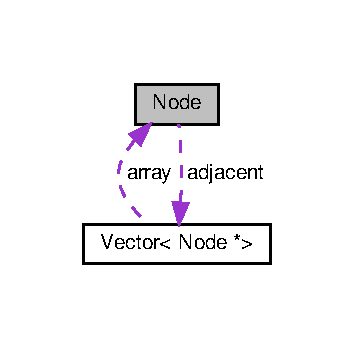
\includegraphics[width=170pt]{classNode__coll__graph}
\end{center}
\end{figure}
\subsection*{Public Member Functions}
\begin{DoxyCompactItemize}
\item 
\mbox{\Hypertarget{classNode_a93070ee4bc38bebbe964a27ca463055b}\label{classNode_a93070ee4bc38bebbe964a27ca463055b}} 
{\bfseries Node} (string s)
\item 
void \hyperlink{classNode_a527dac60fb4649415fc00fe81da91153}{connect} (\hyperlink{classNode}{Node} $\ast$n)
\begin{DoxyCompactList}\small\item\em Connect two nodes. \end{DoxyCompactList}\item 
\mbox{\Hypertarget{classNode_a7c565caad2fea0439f28d24887ac2498}\label{classNode_a7c565caad2fea0439f28d24887ac2498}} 
void {\bfseries reset} ()
\end{DoxyCompactItemize}
\subsection*{Public Attributes}
\begin{DoxyCompactItemize}
\item 
\mbox{\Hypertarget{classNode_a4cd656d544174479df27f0759e5a3997}\label{classNode_a4cd656d544174479df27f0759e5a3997}} 
string {\bfseries name}
\item 
\mbox{\Hypertarget{classNode_a33d398150241451968f5a08ee806a8d7}\label{classNode_a33d398150241451968f5a08ee806a8d7}} 
\hyperlink{classVector}{Vector}$<$ \hyperlink{classNode}{Node} $\ast$ $>$ {\bfseries adjacent}
\item 
\mbox{\Hypertarget{classNode_aa1bdec4e775fc578632e6a2dced9e251}\label{classNode_aa1bdec4e775fc578632e6a2dced9e251}} 
bool {\bfseries visited}
\item 
\mbox{\Hypertarget{classNode_a420f57dad14f36839b73b16454f89608}\label{classNode_a420f57dad14f36839b73b16454f89608}} 
int {\bfseries distance}
\end{DoxyCompactItemize}


\subsection{Detailed Description}
\hyperlink{classNode}{Node} class for tree. 

\subsection{Member Function Documentation}
\mbox{\Hypertarget{classNode_a527dac60fb4649415fc00fe81da91153}\label{classNode_a527dac60fb4649415fc00fe81da91153}} 
\index{Node@{Node}!connect@{connect}}
\index{connect@{connect}!Node@{Node}}
\subsubsection{\texorpdfstring{connect()}{connect()}}
{\footnotesize\ttfamily void Node\+::connect (\begin{DoxyParamCaption}\item[{\hyperlink{classNode}{Node} $\ast$}]{n }\end{DoxyParamCaption})\hspace{0.3cm}{\ttfamily [inline]}}



Connect two nodes. 


\begin{DoxyParams}{Parameters}
{\em n} & \\
\hline
\end{DoxyParams}


The documentation for this class was generated from the following file\+:\begin{DoxyCompactItemize}
\item 
\hyperlink{main_8cpp}{main.\+cpp}\end{DoxyCompactItemize}

\hypertarget{classVector}{}\section{Vector$<$ T $>$ Class Template Reference}
\label{classVector}\index{Vector$<$ T $>$@{Vector$<$ T $>$}}


\hyperlink{classVector}{Vector} class implementation without stl.  


\subsection*{Public Member Functions}
\begin{DoxyCompactItemize}
\item 
\mbox{\Hypertarget{classVector_a3acaa419a1c75e006f15277c1a2eadab}\label{classVector_a3acaa419a1c75e006f15277c1a2eadab}} 
{\bfseries Vector} (int t=10)
\item 
\mbox{\Hypertarget{classVector_aead4cd671608c7210bfa78e748fe5960}\label{classVector_aead4cd671608c7210bfa78e748fe5960}} 
void {\bfseries resize} (int new\+Cap)
\item 
void \hyperlink{classVector_ae20302aab0ca138a87c1541a7f68214d}{push} (T adj)
\begin{DoxyCompactList}\small\item\em Push elements to vector. \end{DoxyCompactList}\item 
\mbox{\Hypertarget{classVector_a5db0910fc60e17551b75f6b227c49b46}\label{classVector_a5db0910fc60e17551b75f6b227c49b46}} 
T \& {\bfseries operator\mbox{[}$\,$\mbox{]}} (int i)
\end{DoxyCompactItemize}
\subsection*{Public Attributes}
\begin{DoxyCompactItemize}
\item 
\mbox{\Hypertarget{classVector_ab6d96ed0a33ffcaa28ecd9b3182a656c}\label{classVector_ab6d96ed0a33ffcaa28ecd9b3182a656c}} 
T $\ast$ {\bfseries array}
\item 
\mbox{\Hypertarget{classVector_a5d3cb041a578dd57f8100e89a798afd6}\label{classVector_a5d3cb041a578dd57f8100e89a798afd6}} 
int {\bfseries count}
\item 
\mbox{\Hypertarget{classVector_a426ffb7c72f7b9dda5457d3bb31e6838}\label{classVector_a426ffb7c72f7b9dda5457d3bb31e6838}} 
int {\bfseries capacity}
\end{DoxyCompactItemize}


\subsection{Detailed Description}
\subsubsection*{template$<$class T$>$\newline
class Vector$<$ T $>$}

\hyperlink{classVector}{Vector} class implementation without stl. 


\begin{DoxyTemplParams}{Template Parameters}
{\em T} & \\
\hline
\end{DoxyTemplParams}


\subsection{Member Function Documentation}
\mbox{\Hypertarget{classVector_ae20302aab0ca138a87c1541a7f68214d}\label{classVector_ae20302aab0ca138a87c1541a7f68214d}} 
\index{Vector@{Vector}!push@{push}}
\index{push@{push}!Vector@{Vector}}
\subsubsection{\texorpdfstring{push()}{push()}}
{\footnotesize\ttfamily template$<$class T$>$ \\
void \hyperlink{classVector}{Vector}$<$ T $>$\+::push (\begin{DoxyParamCaption}\item[{T}]{adj }\end{DoxyParamCaption})\hspace{0.3cm}{\ttfamily [inline]}}



Push elements to vector. 


\begin{DoxyParams}{Parameters}
{\em adj} & \\
\hline
\end{DoxyParams}


The documentation for this class was generated from the following file\+:\begin{DoxyCompactItemize}
\item 
\hyperlink{main_8cpp}{main.\+cpp}\end{DoxyCompactItemize}

\chapter{File Documentation}
\hypertarget{main_8cpp}{}\section{main.\+cpp File Reference}
\label{main_8cpp}\index{main.\+cpp@{main.\+cpp}}


main file for problem 1  


{\ttfamily \#include $<$fstream$>$}\newline
{\ttfamily \#include $<$iostream$>$}\newline
{\ttfamily \#include $<$sstream$>$}\newline
{\ttfamily \#include $<$string$>$}\newline
Include dependency graph for main.\+cpp\+:
\nopagebreak
\begin{figure}[H]
\begin{center}
\leavevmode
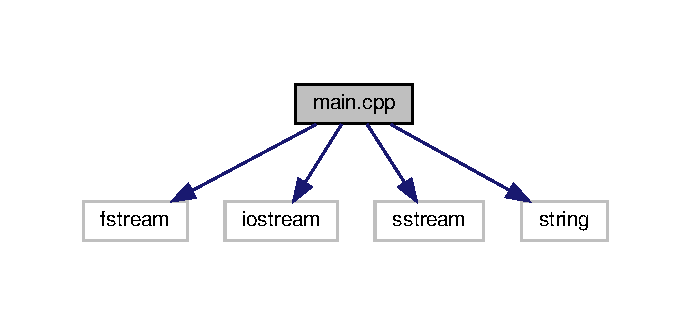
\includegraphics[width=332pt]{main_8cpp__incl}
\end{center}
\end{figure}
\subsection*{Classes}
\begin{DoxyCompactItemize}
\item 
class \hyperlink{classVector}{Vector$<$ T $>$}
\begin{DoxyCompactList}\small\item\em \hyperlink{classVector}{Vector} class implementation without stl. \end{DoxyCompactList}\item 
class \hyperlink{classNode}{Node}
\begin{DoxyCompactList}\small\item\em \hyperlink{classNode}{Node} class for tree. \end{DoxyCompactList}\end{DoxyCompactItemize}
\subsection*{Functions}
\begin{DoxyCompactItemize}
\item 
\hyperlink{classNode}{Node} $\ast$ \hyperlink{main_8cpp_ac05c8fb9a48b8eb20d02ce530b5a77d9}{find\+Node} (string name, \hyperlink{classVector}{Vector}$<$ \hyperlink{classNode}{Node} $>$ \&nodes)
\begin{DoxyCompactList}\small\item\em find node of particular name \end{DoxyCompactList}\item 
void \hyperlink{main_8cpp_a69ceafccb3554e83530d395ee208caa9}{reset\+Nodes} (\hyperlink{classVector}{Vector}$<$ \hyperlink{classNode}{Node} $>$ \&nodes)
\begin{DoxyCompactList}\small\item\em reset all the nodes \end{DoxyCompactList}\item 
bool \hyperlink{main_8cpp_af114394f365b44f910989aa1b5e1d157}{recursive\+Loop\+Find} (\hyperlink{classNode}{Node} $\ast$root, \hyperlink{classNode}{Node} $\ast$parent)
\begin{DoxyCompactList}\small\item\em Finds the loop in graph. \end{DoxyCompactList}\item 
void \hyperlink{main_8cpp_a5e64ea85e86400bd9e4f0f4d37e372a8}{print\+B\+FS} (\hyperlink{classNode}{Node} $\ast$root)
\begin{DoxyCompactList}\small\item\em Print the B\+FS of graph. \end{DoxyCompactList}\item 
void \hyperlink{main_8cpp_a74cea7ac3c0e9a2a66cdcb9ad90655ce}{travel} (\hyperlink{classNode}{Node} $\ast$root, int distance)
\begin{DoxyCompactList}\small\item\em Travel through the graph. \end{DoxyCompactList}\item 
int \hyperlink{main_8cpp_a809575e6915d3f1c1c96a4377685b1ae}{find\+Max\+Distance} (\hyperlink{classVector}{Vector}$<$ \hyperlink{classNode}{Node} $>$ \&nodes)
\begin{DoxyCompactList}\small\item\em find maximum distance in the graph \end{DoxyCompactList}\item 
void \hyperlink{main_8cpp_a7bc0e94fb0ee59c1f5c8d024b38eccdb}{print\+Diameter} (\hyperlink{classVector}{Vector}$<$ \hyperlink{classNode}{Node} $>$ \&nodes)
\begin{DoxyCompactList}\small\item\em prints the diameter of graph \end{DoxyCompactList}\item 
void \hyperlink{main_8cpp_a0fd050dcb16500263f4adae9bf873bf5}{print\+D\+FS} (\hyperlink{classNode}{Node} $\ast$root)
\begin{DoxyCompactList}\small\item\em Prints the D\+FS of graph. \end{DoxyCompactList}\item 
void \hyperlink{main_8cpp_a5aa65c31d6c710646427a8750365bbaa}{parse\+File} (ifstream \&file, \hyperlink{classVector}{Vector}$<$ \hyperlink{classNode}{Node} $>$ \&nodes)
\begin{DoxyCompactList}\small\item\em Parse the input file. \end{DoxyCompactList}\item 
int \hyperlink{main_8cpp_a0ddf1224851353fc92bfbff6f499fa97}{main} (int argc, char $\ast$argv\mbox{[}$\,$\mbox{]})
\begin{DoxyCompactList}\small\item\em main function \end{DoxyCompactList}\end{DoxyCompactItemize}


\subsection{Detailed Description}
main file for problem 1 

\begin{DoxyAuthor}{Author}
Utkarsh 
\end{DoxyAuthor}
\begin{DoxyVersion}{Version}
0.\+1 
\end{DoxyVersion}
\begin{DoxyDate}{Date}
2019-\/10-\/09
\end{DoxyDate}
\begin{DoxyCopyright}{Copyright}
Copyright (c) 2019 
\end{DoxyCopyright}


\subsection{Function Documentation}
\mbox{\Hypertarget{main_8cpp_a809575e6915d3f1c1c96a4377685b1ae}\label{main_8cpp_a809575e6915d3f1c1c96a4377685b1ae}} 
\index{main.\+cpp@{main.\+cpp}!find\+Max\+Distance@{find\+Max\+Distance}}
\index{find\+Max\+Distance@{find\+Max\+Distance}!main.\+cpp@{main.\+cpp}}
\subsubsection{\texorpdfstring{find\+Max\+Distance()}{findMaxDistance()}}
{\footnotesize\ttfamily int find\+Max\+Distance (\begin{DoxyParamCaption}\item[{\hyperlink{classVector}{Vector}$<$ \hyperlink{classNode}{Node} $>$ \&}]{nodes }\end{DoxyParamCaption})}



find maximum distance in the graph 


\begin{DoxyParams}{Parameters}
{\em nodes} & \\
\hline
\end{DoxyParams}
\begin{DoxyReturn}{Returns}
int 
\end{DoxyReturn}
\mbox{\Hypertarget{main_8cpp_ac05c8fb9a48b8eb20d02ce530b5a77d9}\label{main_8cpp_ac05c8fb9a48b8eb20d02ce530b5a77d9}} 
\index{main.\+cpp@{main.\+cpp}!find\+Node@{find\+Node}}
\index{find\+Node@{find\+Node}!main.\+cpp@{main.\+cpp}}
\subsubsection{\texorpdfstring{find\+Node()}{findNode()}}
{\footnotesize\ttfamily \hyperlink{classNode}{Node}$\ast$ find\+Node (\begin{DoxyParamCaption}\item[{string}]{name,  }\item[{\hyperlink{classVector}{Vector}$<$ \hyperlink{classNode}{Node} $>$ \&}]{nodes }\end{DoxyParamCaption})}



find node of particular name 


\begin{DoxyParams}{Parameters}
{\em name} & \\
\hline
{\em nodes} & \\
\hline
\end{DoxyParams}
\begin{DoxyReturn}{Returns}
Node$\ast$ 
\end{DoxyReturn}
\mbox{\Hypertarget{main_8cpp_a0ddf1224851353fc92bfbff6f499fa97}\label{main_8cpp_a0ddf1224851353fc92bfbff6f499fa97}} 
\index{main.\+cpp@{main.\+cpp}!main@{main}}
\index{main@{main}!main.\+cpp@{main.\+cpp}}
\subsubsection{\texorpdfstring{main()}{main()}}
{\footnotesize\ttfamily int main (\begin{DoxyParamCaption}\item[{int}]{argc,  }\item[{char $\ast$}]{argv\mbox{[}$\,$\mbox{]} }\end{DoxyParamCaption})}



main function 


\begin{DoxyParams}{Parameters}
{\em argc} & \\
\hline
{\em argv} & \\
\hline
\end{DoxyParams}
\begin{DoxyReturn}{Returns}
int 
\end{DoxyReturn}
\mbox{\Hypertarget{main_8cpp_a5aa65c31d6c710646427a8750365bbaa}\label{main_8cpp_a5aa65c31d6c710646427a8750365bbaa}} 
\index{main.\+cpp@{main.\+cpp}!parse\+File@{parse\+File}}
\index{parse\+File@{parse\+File}!main.\+cpp@{main.\+cpp}}
\subsubsection{\texorpdfstring{parse\+File()}{parseFile()}}
{\footnotesize\ttfamily void parse\+File (\begin{DoxyParamCaption}\item[{ifstream \&}]{file,  }\item[{\hyperlink{classVector}{Vector}$<$ \hyperlink{classNode}{Node} $>$ \&}]{nodes }\end{DoxyParamCaption})}



Parse the input file. 


\begin{DoxyParams}{Parameters}
{\em file} & \\
\hline
{\em nodes} & \\
\hline
\end{DoxyParams}
\mbox{\Hypertarget{main_8cpp_a5e64ea85e86400bd9e4f0f4d37e372a8}\label{main_8cpp_a5e64ea85e86400bd9e4f0f4d37e372a8}} 
\index{main.\+cpp@{main.\+cpp}!print\+B\+FS@{print\+B\+FS}}
\index{print\+B\+FS@{print\+B\+FS}!main.\+cpp@{main.\+cpp}}
\subsubsection{\texorpdfstring{print\+B\+F\+S()}{printBFS()}}
{\footnotesize\ttfamily void print\+B\+FS (\begin{DoxyParamCaption}\item[{\hyperlink{classNode}{Node} $\ast$}]{root }\end{DoxyParamCaption})}



Print the B\+FS of graph. 


\begin{DoxyParams}{Parameters}
{\em root} & \\
\hline
\end{DoxyParams}
\mbox{\Hypertarget{main_8cpp_a0fd050dcb16500263f4adae9bf873bf5}\label{main_8cpp_a0fd050dcb16500263f4adae9bf873bf5}} 
\index{main.\+cpp@{main.\+cpp}!print\+D\+FS@{print\+D\+FS}}
\index{print\+D\+FS@{print\+D\+FS}!main.\+cpp@{main.\+cpp}}
\subsubsection{\texorpdfstring{print\+D\+F\+S()}{printDFS()}}
{\footnotesize\ttfamily void print\+D\+FS (\begin{DoxyParamCaption}\item[{\hyperlink{classNode}{Node} $\ast$}]{root }\end{DoxyParamCaption})}



Prints the D\+FS of graph. 


\begin{DoxyParams}{Parameters}
{\em root} & \\
\hline
\end{DoxyParams}
\mbox{\Hypertarget{main_8cpp_a7bc0e94fb0ee59c1f5c8d024b38eccdb}\label{main_8cpp_a7bc0e94fb0ee59c1f5c8d024b38eccdb}} 
\index{main.\+cpp@{main.\+cpp}!print\+Diameter@{print\+Diameter}}
\index{print\+Diameter@{print\+Diameter}!main.\+cpp@{main.\+cpp}}
\subsubsection{\texorpdfstring{print\+Diameter()}{printDiameter()}}
{\footnotesize\ttfamily void print\+Diameter (\begin{DoxyParamCaption}\item[{\hyperlink{classVector}{Vector}$<$ \hyperlink{classNode}{Node} $>$ \&}]{nodes }\end{DoxyParamCaption})}



prints the diameter of graph 


\begin{DoxyParams}{Parameters}
{\em nodes} & \\
\hline
\end{DoxyParams}
\mbox{\Hypertarget{main_8cpp_af114394f365b44f910989aa1b5e1d157}\label{main_8cpp_af114394f365b44f910989aa1b5e1d157}} 
\index{main.\+cpp@{main.\+cpp}!recursive\+Loop\+Find@{recursive\+Loop\+Find}}
\index{recursive\+Loop\+Find@{recursive\+Loop\+Find}!main.\+cpp@{main.\+cpp}}
\subsubsection{\texorpdfstring{recursive\+Loop\+Find()}{recursiveLoopFind()}}
{\footnotesize\ttfamily bool recursive\+Loop\+Find (\begin{DoxyParamCaption}\item[{\hyperlink{classNode}{Node} $\ast$}]{root,  }\item[{\hyperlink{classNode}{Node} $\ast$}]{parent }\end{DoxyParamCaption})}



Finds the loop in graph. 


\begin{DoxyParams}{Parameters}
{\em root} & \\
\hline
{\em parent} & \\
\hline
\end{DoxyParams}
\begin{DoxyReturn}{Returns}
true 

false 
\end{DoxyReturn}
\mbox{\Hypertarget{main_8cpp_a69ceafccb3554e83530d395ee208caa9}\label{main_8cpp_a69ceafccb3554e83530d395ee208caa9}} 
\index{main.\+cpp@{main.\+cpp}!reset\+Nodes@{reset\+Nodes}}
\index{reset\+Nodes@{reset\+Nodes}!main.\+cpp@{main.\+cpp}}
\subsubsection{\texorpdfstring{reset\+Nodes()}{resetNodes()}}
{\footnotesize\ttfamily void reset\+Nodes (\begin{DoxyParamCaption}\item[{\hyperlink{classVector}{Vector}$<$ \hyperlink{classNode}{Node} $>$ \&}]{nodes }\end{DoxyParamCaption})}



reset all the nodes 


\begin{DoxyParams}{Parameters}
{\em nodes} & \\
\hline
\end{DoxyParams}
\mbox{\Hypertarget{main_8cpp_a74cea7ac3c0e9a2a66cdcb9ad90655ce}\label{main_8cpp_a74cea7ac3c0e9a2a66cdcb9ad90655ce}} 
\index{main.\+cpp@{main.\+cpp}!travel@{travel}}
\index{travel@{travel}!main.\+cpp@{main.\+cpp}}
\subsubsection{\texorpdfstring{travel()}{travel()}}
{\footnotesize\ttfamily void travel (\begin{DoxyParamCaption}\item[{\hyperlink{classNode}{Node} $\ast$}]{root,  }\item[{int}]{distance }\end{DoxyParamCaption})}



Travel through the graph. 


\begin{DoxyParams}{Parameters}
{\em root} & \\
\hline
{\em distance} & \\
\hline
\end{DoxyParams}

%--- End generated contents ---

% Index
\backmatter
\newpage
\phantomsection
\clearemptydoublepage
\addcontentsline{toc}{chapter}{Index}
\printindex

\end{document}
